\subsection{Protein Synthesis}
The last process of the central dogma -- the translation of RNA into 
protein -- is the final subject in our dialogue between back-of-the-envelope
estimates and comparison with proteomic data.
% becomes the next and final subject for our back-of-the-envelope
% estimates.
Here we consider the number of ribosomes needed to replicate the cellular
proteome.  While the rate at which ribosomes translates is well known to have a
growth rate dependence \cite{dai2018}, here we make the approximation that
translation occurs at a rate of $\approx$ 15 amino acids per second per ribosome
(BNID: 100233). Under this approximation and assuming a division time of 5000 s,
we can easily arrive at an estimate of $\approx 10^4$ ribosomes needed to
replicate the entire protein mass (\FIG{protein_synthesis}). This point estimate
and the corresponding estimate across a continuum of growth rates proves to be
notably comparable to the experimental observations, shown in
\FIG{protein_synthesis}(B). While the ribosome is responsible for the formation
of peptide bonds, we do not diminish the importance of the charging of tRNAs
with the appropriate amino acid, a process with occurs with remarkable accuracy.
In the Appendix and in \FIGSUPP[protein_synthesis]{tRNA}, we consider the
process of ligating tRNAs to their corresponding amino acid and again find
notable comparability with the data.


%While this is a critical step
%in protein synthesis whose efficiency reflects the nutritional richness of the
%growth medium, the ability to parallelize this process by expressing more tRNA
%ligases makes it unlikely to be a bottleneck for cell division.


% We will begin our exploration of protein translation in the same spirit as in
% previous sections with an estimate of the number of ribosomes needed to
% replicate the proteome.
% Ribosomes are enormous
% protein/rRNA complexes that facilitate the peptide bond formation between amino
% acids in the correct sequence as defined by the coding mRNA. Before we examine
% the synthesis of the ribosome proteins and the limits that may place on the
% observed bacterial growth rates, let's consider replication of the cellular
% proteome.
% is a topic which we discuss in detail in
% the coming sections. However, for the purposes of our order-of-magnitude
% estimate, we can
% , while
% glossing over important details such as chromosome copy number and
% growth-rate dependent translation rates,

\begin{figure}
    \centering{
        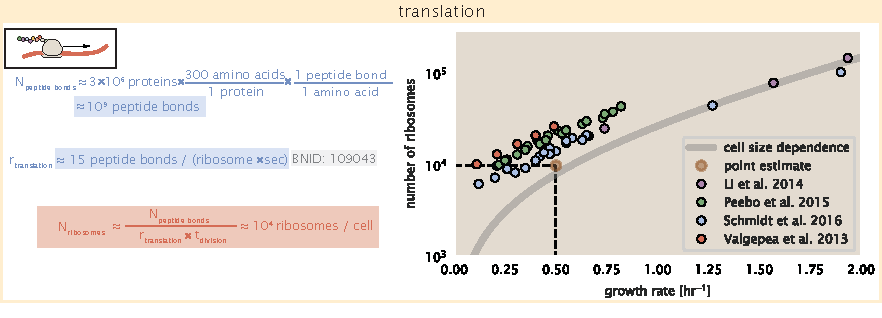
\includegraphics{main_figs/protein_synthesis_main.pdf}
    }
        \caption{\textbf{Estimation of the required number of ribosomes.} Estimation of the
        number of ribosomes required to synthesize 10$^9$ peptide bonds with an
        elongation rate of 15 peptide bonds per second. The
        average abundance of ribosomes is plotted as a function of growth rate.
        Our estimated values are shown for a growth rate of 0.5 hr$^{-1}$.
        Grey lines correspond to the estimated complex abundance calculated at
        different growth rates.} \label{fig:protein_synthesis}

        \figsupp[Estimate and observed abundance and growth rate dependence
        of tRNA ligases.]{Estimation for the number of tRNA synthetases that
        will supply the required amino acid demand. The sum of all tRNA
        synthetases copy numbers are plotted as a function of growth rate
        ([ArgS], [CysS], [GlnS], [GltX], [IleS], [LeuS], [ValS], [AlaS]$_2$,
        [AsnS]$_2$, [AspS]$_2$, [TyrS]$_2$, [TrpS]$_2$, [ThrS]$_2$,
        [SerS]$_2$, [ProS]$_2$, [PheS]$_2$[PheT]$_2$, [MetG]$_2$,
        [lysS]$_2$, [HisS]$_2$, [GlyS]$_2$[GlyQ]$_2$).}{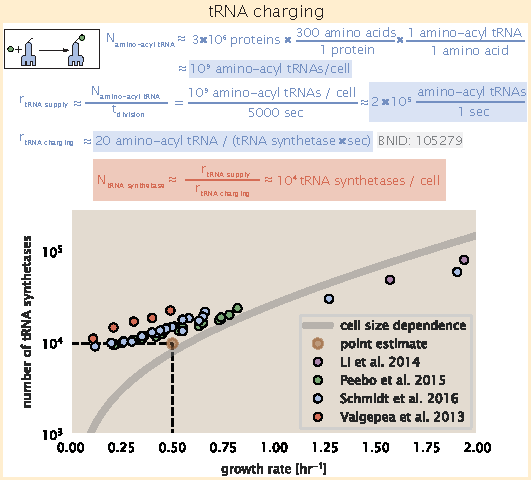
\includegraphics{main_figs/tRNA.pdf}}\label{figsupp:tRNA}
\end{figure}
